\documentclass[11pt]{article}
\usepackage{fullpage}
\usepackage{verbatim}
\usepackage{moreverb}
\usepackage{amsmath}
\let\verbatiminput=\verbatimtabinput
\def\verbatimtabsize{4\relax}
\usepackage{tikz}
\usetikzlibrary{arrows,automata, positioning}
\usepackage{array}
\usepackage{booktabs}
\usepackage{minted}
\usepackage{parskip}
\usepackage{float}
\usepackage{pbox}
\usepackage{makecell}
\graphicspath{{images/}}

\usepackage{color}
\definecolor{rltred}{rgb}{0.75,0,0}
\definecolor{rltgreen}{rgb}{0,0.5,0}
\definecolor{rltblue}{rgb}{0,0,0.75}

\usepackage[%pdftex,
    colorlinks=true,
    urlcolor=rltblue,               % \href{...}{...}
    anchorcolor=rltbrightblue,
    filecolor=rltgreen,             % \href*{...}
    linkcolor=rltred,               % \ref{...} and \pageref{...}
    menucolor=webdarkblue,
    citecolor=webbrightgreen,
    pagebackref,
    pdfpagemode=UseNone,
    bookmarksopen=true]{hyperref}
\usepackage{graphicx}
\usepackage{hyperref}

\newcommand{\itwos}{I\textsuperscript{2}S}

\newcommand{\instbit}[1]{\mbox{\scriptsize #1}}
\newcommand{\instbitrange}[2]{~\instbit{#1} \hfill \instbit{#2}~}

\newcommand{\currentSemester}{Fall 2019}
\newcommand{\projectSpecVersion}{4.3}

\newcommand{\dueDateTime}{end of lab sessions}

\newcommand{\blockDiagramTaskName}{Checkpoint 1}
\newcommand{\blockDiagramDueDate}{November 1}
\newcommand{\blockDiagramTimeAlloted}{1 week}

\newcommand{\baseCPUTaskName}{Checkpoint 2}
\newcommand{\baseCPUDueDate}{November 22}
\newcommand{\baseCPUTimeAlloted}{3 weeks}

\newcommand{\audioTaskName}{Checkpoint 3}
\newcommand{\audioDueDate}{December 9}
\newcommand{\audioTimeAlloted}{2 weeks}

\newcommand{\dfsTaskName}{Checkpoint 4}
\newcommand{\dfsDueDate}{December 6}
\newcommand{\dfsTimeAlloted}{2 weeks}

\newcommand{\finalCheckoffDueDate}{December 9 (by appointment)}

\newcommand{\finalReportDueDate}{December 11}

\newcommand{\skeletonRepoName}{project\_skeleton\_fa19}
\newcommand{\semesterName}{fa19}

%Also, change the info in minted blocks.  This includes the "Setting up your Code Repository" section and the "Setting up the Vivado Project" section


\begin{document}
\begin{center}
{\bf
University of California at Berkeley \\
College of Engineering \\
Department of Electrical Engineering and Computer Science \\
}
\end{center}

\begin{center}
EECS151/251A - LB, \currentSemester
\end{center}

\begin{center}
\LARGE
{\bf Project Specification: RISCV151 }  \\
Version \projectSpecVersion
\end{center}

\tableofcontents

\newpage

\section{Introduction}
The goal of this project is to familiarize EECS151/251A students with the methods and tools of digital design.
In teams of 2, you will design and implement a 3-stage pipelined RISC-V CPU with a UART for tethering.
Afterwards, you will attach the IO circuits you built in the lab to the CPU and design a subtractive audio synthesizer.
Then, you will implement a simple dynamic frequency scaling algorithm to bound the power consumption and temperature of your FPGA design while achieving a performance target.
Finally, you will optimize your CPU for performance (maximizing the Iron Law) and cost (FPGA resource utilization).

You will use Verilog to implement this system, targeting the Xilinx Pynq platform (a Pynq-Z1 development board with a Zynq 7000-series FPGA).
The project will give you experience designing with RTL descriptions, resolving hazards in a simple pipeline, building interfaces, and teach you how to approach system-level optimization.

In tackling these challenges, your first step will be to map the high level specification to a design which can be translated into a hardware implementation.
After that, you will produce and debug that implementation.
These first steps can take significant time if you have not thought out your design prior to trying implementation.

As in previous semesters, your EECS151/251A project is probably the largest project you have faced so far here at Berkeley.
Good time management and good design organization is critical to your success.

\subsection{Tentative Deadlines}
\label{tentative_deadlines}
The following is a brief description of each checkpoint and approximately how many weeks will be alloted to each one. This schedule may change as the semester progresses. The current schedule is summarised at the end of the document in Section \ref{project_timeline}.

\begin{itemize}
  \item \textbf{\blockDiagramDueDate \space - \blockDiagramTaskName \space (\blockDiagramTimeAlloted)} - Draw a schematic of your processor's datapath and pipeline stages.
  \item \textbf{\baseCPUDueDate \space - \baseCPUTaskName \space (\baseCPUTimeAlloted)} - Implement your RISC-V processor core in Verilog and write tests to verify your implementation.
  \item \textbf{\audioDueDate \space - \audioTaskName \space (\audioTimeAlloted)} - Attach I/O components from lab to your processor (FIFOs, buttons, switches), general PWM controller, basic subtractive synthesizer
  \item \textbf{\dfsDueDate \space - \dfsTaskName \space (\dfsTimeAlloted)} - Implement a dedicated power management unit to monitor FPGA temperature and power consumption and dynamically switch the operating frequency of the main CPU.
  \item \textbf{\finalCheckoffDueDate \space - Final Checkoff} - Final processor optimization and checkoff
  \item \textbf{\finalReportDueDate \space - Project Report} - Final report due
\end{itemize}

\subsection{General Project Tips}
\label{tips}
Document your project as you go.
You should comment your Verilog and keep your diagrams up to date.
Aside from the final project report (you will need to turn in a report documenting your project), you can use your design documents to help the debugging process.

Finish the required features first.
Attempt extra features after everything works well.
\textbf{If your submitted project does not work by the final deadline, you will not get any credit for any extra credit features you have implemented.}

This project, as has been done in past semesters, will be divided into checkpoints. The following sections will specify the objectives for each checkpoint.

\section{Checkpoints 1 \& 2 - 3-stage Pipelined RISC-V CPU}
The first checkpoint in this project is designed to guide the development of a three-stage pipelined RISC-V CPU that will be used as a base system in subsequent checkpoints.

\textbf{TODO: REPLACE THIS DIAGRAM}
\begin{figure}[hbt]
\begin{center}
  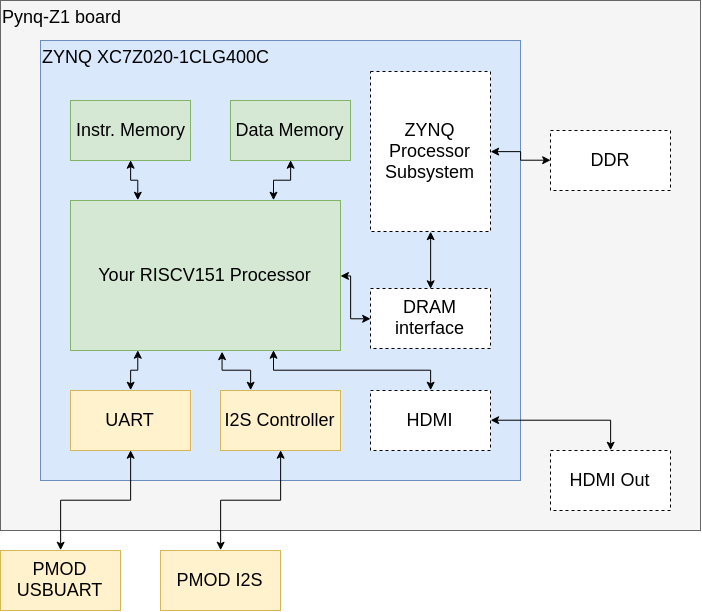
\includegraphics[width=4in]{riscv151overview.png}
  \caption{High-level overview of the full system}
  \label{fig:sys_overview}
\end{center}
\end{figure}

The green (RISC-V core) and yellow (UART/counters) blocks on the diagram are the focus of the first and second checkpoints.
The third checkpoint will add audio and IO components in blue.
Finally, the fourth checkpoint will implement the power management unit in red.

\subsection{Setting up your Code Repository}
The project skeleton files are available on Github.
The suggested way for initializing your repository with the skeleton files is as follows:

\begin{minted}[tabsize=2]{bash}
  git clone git@github.com:EECS150/project_skeleton_fa19.git
  cd project_skeleton_fa19
  git remote add my-repo git@github.com:EECS150/fa19_teamXX.git
  git push my-repo master
\end{minted}

Then reclone your repo and add the skeleton repo as a remote:
\begin{minted}[tabsize=2]{bash}
  cd ..
  rm -rf project_skeleton_fa19
  git clone git@github.com:EECS150/fa19_teamXX.git
  cd fa19_teamXX
  git remote add staff git@github.com:EECS150/project_skeleton_fa19.git
\end{minted}

To pull project updates from the skeleton repo, run \verb|git pull staff master|.

To get a team repo, fill one line in the Google spreadsheet posted on Piazza with your team information (names, Github logins, and enrolled lab session).

You should check frequently for updates to the skeleton files.
Update announcements will be posted to Piazza.

\subsection{Integrate Designs from Labs} \label{past_designs}
You should copy some modules you designed from the labs.
We suggest you keep these with the provided source files in \verb|hardware/src| (overwriting any provided skeletons).

\begin{minted}[tabsize=2]{bash}
  cd fa19_teamXX
  cp fpga_labs_fa19/lab6/debouncer.v fa19_teamXX/hardware/src/io_circuits/.
\end{minted}

\textbf{Copy these files from the labs:}
\begin{minted}{bash}
  lab6/debouncer.v
  lab6/synchronizer.v
  lab6/edge_detector.v
  lab6/fifo.v
  lab6/uart_transmitter.v
\end{minted}

\subsection{Project Skeleton Overview}
\begin{itemize}
  \item \texttt{hardware}
    \begin{itemize}
      \item \texttt{src}
        \begin{itemize}
          \item \texttt{z1top.v}: Top level module. The RISC-V CPU is instantiated here.
          \item \texttt{PYNQ-Z1.xdc}: Constraints file. You can modify this to change pin assignments for peripherals when connecting I/O.
          \item \texttt{riscv\_core/Riscv151.v}: All of your CPU datapath and control should be contained in this file.
          \item \texttt{riscv\_core/reg\_file.v}: Your register file implementation.
          \item \verb|memories/{imem, dmem, bios_mem}.v|: Synthesizable RAMs for the instruction, data, and BIOS memories.
          \item \verb|io_circuits/uart.v, uart_transmitter.v, uart_receiver.v|: Your working UART from Labs 5 and 6
        \end{itemize}
      \item \texttt{sim}
        \begin{itemize}
          \item \verb|assembly_testbench.v|: Starting point for testing your CPU. Works with the software in \texttt{assembly\_tests}.
          \item \verb|echo_testbench.v|: Runs the software in \texttt{echo} on your CPU. The software implements the echo FSM from lab 5, and the testbench controls an off-chip UART to test it.
        \end{itemize}
    \end{itemize}
  \item \texttt{software}
    \begin{itemize}
      \item \verb|bios151v3|: The BIOS program, which allows us to interact with our CPU via the UART. You need to compile it compile it before creating a bitstream or running a simulation.
      \item \verb|echo|: The echo program, which emulates the FSM from Lab 5 in software.
      \item \verb|assembly_tests|: Use this as a template to write assembly tests for your processor designed to run in simulation.
      \item \verb|c_example|: Use this as an example to write C programs.
      \item \verb|mmult|: This is a program to be run on the FPGA for Checkpoint 2. It generates 2 matrices and multiplies them. Then it returns a checksum to verify the correct result.
    \end{itemize}
\end{itemize}

To compile \texttt{software} go into a program directory and run \texttt{make}.
To build a bitstream run \texttt{make impl} in \texttt{hardware}.

\subsection{RISC-V 151 ISA}
Table \ref{tab:ISA} contains all of the instructions your processor is responsible for supporting.
It contains most of the instructions specified in the RV32I Base Instruction set, and allows us to maintain a relatively simple design while still being able to have a C compiler and write interesting programs to run on the processor.
For the specific details of each instruction, refer to sections 2.2 through 2.6 in the \href{http://riscv.org/specifications/}{RISC-V Instruction Set Manual}.

You may find a \href{https://github.com/jameslzhu/riscv-card/blob/master/riscv-card.pdf}{RISC-V green card} helpful.

\subsubsection{CSR Instructions}
You will have to implement 2 CSR instructions to support running the standard RISC-V ISA test suite.
A CSR (or control status register) is some state that is stored independent of the register file and the memory.
While there are $2^{12}$ possible CSR addresses, you will only use one of them (\texttt{tohost = 0x51E}).
The \texttt{tohost} register is monitored by the RISC-V ISA testbench, and simulation ends when a value is written to this register.
A value of 1 indicates success, a value greater than 1 gives clues as to the location of the failure.

There are 2 CSR related instructions that you will need to implement:
\begin{enumerate}
\item \texttt{csrw tohost,t2}  (short for \texttt{csrrw x0,csr,rs1} where \texttt{csr = 0x51E})
\item \texttt{csrwi tohost,1}  (short for \texttt{csrrwi x0,csr,uimm} where \texttt{csr = 0x51E})
\end{enumerate}

\texttt{csrw} will write the value from register in rs1.
\texttt{csrwi} will write the immediate (stored in rs1) to the addressed csr.
Note that you do not need to write to rd (writing to x0 does nothing).

\begin{table}[p]
\caption{RISC-V ISA}
\label{tab:ISA}
\begin{small}
\begin{center}
\begin{tabular}{p{0in}p{0.4in}p{0.05in}p{0.05in}p{0.05in}p{0.05in}p{0.4in}p{0.6in}p{0.4in}p{0.6in}p{0.7in}l}
& & & & & & & & & & \\
                      &
\multicolumn{1}{l}{\instbit{31}} &
\multicolumn{1}{r}{\instbit{27}} &
\instbit{26} &
\instbit{25} &
\multicolumn{1}{l}{\instbit{24}} &
\multicolumn{1}{r}{\instbit{20}} &
\instbitrange{19}{15} &
\instbitrange{14}{12} &
\instbitrange{11}{7} &
\instbitrange{6}{0} \\
\cline{2-11}


&
\multicolumn{4}{|c|}{funct7} &
\multicolumn{2}{c|}{rs2} &
\multicolumn{1}{c|}{rs1} &
\multicolumn{1}{c|}{funct3} &
\multicolumn{1}{c|}{rd} &
\multicolumn{1}{c|}{opcode} & R-type \\
\cline{2-11}


&
\multicolumn{6}{|c|}{imm[11:0]} &
\multicolumn{1}{c|}{rs1} &
\multicolumn{1}{c|}{funct3} &
\multicolumn{1}{c|}{rd} &
\multicolumn{1}{c|}{opcode} & I-type \\
\cline{2-11}


&
\multicolumn{4}{|c|}{imm[11:5]} &
\multicolumn{2}{c|}{rs2} &
\multicolumn{1}{c|}{rs1} &
\multicolumn{1}{c|}{funct3} &
\multicolumn{1}{c|}{imm[4:0]} &
\multicolumn{1}{c|}{opcode} & S-type \\
\cline{2-11}


&
\multicolumn{4}{|c|}{imm[12$\vert$10:5]} &
\multicolumn{2}{c|}{rs2} &
\multicolumn{1}{c|}{rs1} &
\multicolumn{1}{c|}{funct3} &
\multicolumn{1}{c|}{imm[4:1$\vert$11]} &
\multicolumn{1}{c|}{opcode} & B-type \\
\cline{2-11}


&
\multicolumn{8}{|c|}{imm[31:12]} &
\multicolumn{1}{c|}{rd} &
\multicolumn{1}{c|}{opcode} & U-type \\
\cline{2-11}


&
\multicolumn{8}{|c|}{imm[20$\vert$10:1$\vert$11$\vert$19:12]} &
\multicolumn{1}{c|}{rd} &
\multicolumn{1}{c|}{opcode} & J-type \\
\cline{2-11}


&
\multicolumn{10}{c}{} & \\
&
\multicolumn{10}{c}{\bf RV32I Base Instruction Set} & \\
\cline{2-11}


&
\multicolumn{8}{|c|}{imm[31:12]} &
\multicolumn{1}{c|}{rd} &
\multicolumn{1}{c|}{0110111} & LUI \\
\cline{2-11}


&
\multicolumn{8}{|c|}{imm[31:12]} &
\multicolumn{1}{c|}{rd} &
\multicolumn{1}{c|}{0010111} & AUIPC \\
\cline{2-11}


&
\multicolumn{8}{|c|}{imm[20$\vert$10:1$\vert$11$\vert$19:12]} &
\multicolumn{1}{c|}{rd} &
\multicolumn{1}{c|}{1101111} & JAL \\
\cline{2-11}


&
\multicolumn{6}{|c|}{imm[11:0]} &
\multicolumn{1}{c|}{rs1} &
\multicolumn{1}{c|}{000} &
\multicolumn{1}{c|}{rd} &
\multicolumn{1}{c|}{1100111} & JALR \\
\cline{2-11}


&
\multicolumn{4}{|c|}{imm[12$\vert$10:5]} &
\multicolumn{2}{c|}{rs2} &
\multicolumn{1}{c|}{rs1} &
\multicolumn{1}{c|}{000} &
\multicolumn{1}{c|}{imm[4:1$\vert$11]} &
\multicolumn{1}{c|}{1100011} & BEQ \\
\cline{2-11}


&
\multicolumn{4}{|c|}{imm[12$\vert$10:5]} &
\multicolumn{2}{c|}{rs2} &
\multicolumn{1}{c|}{rs1} &
\multicolumn{1}{c|}{001} &
\multicolumn{1}{c|}{imm[4:1$\vert$11]} &
\multicolumn{1}{c|}{1100011} & BNE \\
\cline{2-11}


&
\multicolumn{4}{|c|}{imm[12$\vert$10:5]} &
\multicolumn{2}{c|}{rs2} &
\multicolumn{1}{c|}{rs1} &
\multicolumn{1}{c|}{100} &
\multicolumn{1}{c|}{imm[4:1$\vert$11]} &
\multicolumn{1}{c|}{1100011} & BLT \\
\cline{2-11}


&
\multicolumn{4}{|c|}{imm[12$\vert$10:5]} &
\multicolumn{2}{c|}{rs2} &
\multicolumn{1}{c|}{rs1} &
\multicolumn{1}{c|}{101} &
\multicolumn{1}{c|}{imm[4:1$\vert$11]} &
\multicolumn{1}{c|}{1100011} & BGE \\
\cline{2-11}


&
\multicolumn{4}{|c|}{imm[12$\vert$10:5]} &
\multicolumn{2}{c|}{rs2} &
\multicolumn{1}{c|}{rs1} &
\multicolumn{1}{c|}{110} &
\multicolumn{1}{c|}{imm[4:1$\vert$11]} &
\multicolumn{1}{c|}{1100011} & BLTU \\
\cline{2-11}


&
\multicolumn{4}{|c|}{imm[12$\vert$10:5]} &
\multicolumn{2}{c|}{rs2} &
\multicolumn{1}{c|}{rs1} &
\multicolumn{1}{c|}{111} &
\multicolumn{1}{c|}{imm[4:1$\vert$11]} &
\multicolumn{1}{c|}{1100011} & BGEU \\
\cline{2-11}


&
\multicolumn{6}{|c|}{imm[11:0]} &
\multicolumn{1}{c|}{rs1} &
\multicolumn{1}{c|}{000} &
\multicolumn{1}{c|}{rd} &
\multicolumn{1}{c|}{0000011} & LB \\
\cline{2-11}


&
\multicolumn{6}{|c|}{imm[11:0]} &
\multicolumn{1}{c|}{rs1} &
\multicolumn{1}{c|}{001} &
\multicolumn{1}{c|}{rd} &
\multicolumn{1}{c|}{0000011} & LH \\
\cline{2-11}


&
\multicolumn{6}{|c|}{imm[11:0]} &
\multicolumn{1}{c|}{rs1} &
\multicolumn{1}{c|}{010} &
\multicolumn{1}{c|}{rd} &
\multicolumn{1}{c|}{0000011} & LW \\
\cline{2-11}


&
\multicolumn{6}{|c|}{imm[11:0]} &
\multicolumn{1}{c|}{rs1} &
\multicolumn{1}{c|}{100} &
\multicolumn{1}{c|}{rd} &
\multicolumn{1}{c|}{0000011} & LBU \\
\cline{2-11}


&
\multicolumn{6}{|c|}{imm[11:0]} &
\multicolumn{1}{c|}{rs1} &
\multicolumn{1}{c|}{101} &
\multicolumn{1}{c|}{rd} &
\multicolumn{1}{c|}{0000011} & LHU \\
\cline{2-11}


&
\multicolumn{4}{|c|}{imm[11:5]} &
\multicolumn{2}{c|}{rs2} &
\multicolumn{1}{c|}{rs1} &
\multicolumn{1}{c|}{000} &
\multicolumn{1}{c|}{imm[4:0]} &
\multicolumn{1}{c|}{0100011} & SB \\
\cline{2-11}


&
\multicolumn{4}{|c|}{imm[11:5]} &
\multicolumn{2}{c|}{rs2} &
\multicolumn{1}{c|}{rs1} &
\multicolumn{1}{c|}{001} &
\multicolumn{1}{c|}{imm[4:0]} &
\multicolumn{1}{c|}{0100011} & SH \\
\cline{2-11}

&
\multicolumn{4}{|c|}{imm[11:5]} &
\multicolumn{2}{c|}{rs2} &
\multicolumn{1}{c|}{rs1} &
\multicolumn{1}{c|}{010} &
\multicolumn{1}{c|}{imm[4:0]} &
\multicolumn{1}{c|}{0100011} & SW \\
\cline{2-11}

&
\multicolumn{6}{|c|}{imm[11:0]} &
\multicolumn{1}{c|}{rs1} &
\multicolumn{1}{c|}{000} &
\multicolumn{1}{c|}{rd} &
\multicolumn{1}{c|}{0010011} & ADDI \\
\cline{2-11}

&
\multicolumn{6}{|c|}{imm[11:0]} &
\multicolumn{1}{c|}{rs1} &
\multicolumn{1}{c|}{010} &
\multicolumn{1}{c|}{rd} &
\multicolumn{1}{c|}{0010011} & SLTI \\
\cline{2-11}

&
\multicolumn{6}{|c|}{imm[11:0]} &
\multicolumn{1}{c|}{rs1} &
\multicolumn{1}{c|}{011} &
\multicolumn{1}{c|}{rd} &
\multicolumn{1}{c|}{0010011} & SLTIU \\
\cline{2-11}

&
\multicolumn{6}{|c|}{imm[11:0]} &
\multicolumn{1}{c|}{rs1} &
\multicolumn{1}{c|}{100} &
\multicolumn{1}{c|}{rd} &
\multicolumn{1}{c|}{0010011} & XORI \\
\cline{2-11}

&
\multicolumn{6}{|c|}{imm[11:0]} &
\multicolumn{1}{c|}{rs1} &
\multicolumn{1}{c|}{110} &
\multicolumn{1}{c|}{rd} &
\multicolumn{1}{c|}{0010011} & ORI \\
\cline{2-11}

&
\multicolumn{6}{|c|}{imm[11:0]} &
\multicolumn{1}{c|}{rs1} &
\multicolumn{1}{c|}{111} &
\multicolumn{1}{c|}{rd} &
\multicolumn{1}{c|}{0010011} & ANDI \\
\cline{2-11}

&
\multicolumn{4}{|c|}{0000000} &
\multicolumn{2}{c|}{shamt} &
\multicolumn{1}{c|}{rs1} &
\multicolumn{1}{c|}{001} &
\multicolumn{1}{c|}{rd} &
\multicolumn{1}{c|}{0010011} & SLLI \\
\cline{2-11}

&
\multicolumn{4}{|c|}{0000000} &
\multicolumn{2}{c|}{shamt} &
\multicolumn{1}{c|}{rs1} &
\multicolumn{1}{c|}{101} &
\multicolumn{1}{c|}{rd} &
\multicolumn{1}{c|}{0010011} & SRLI \\
\cline{2-11}

&
\multicolumn{4}{|c|}{0100000} &
\multicolumn{2}{c|}{shamt} &
\multicolumn{1}{c|}{rs1} &
\multicolumn{1}{c|}{101} &
\multicolumn{1}{c|}{rd} &
\multicolumn{1}{c|}{0010011} & SRAI \\
\cline{2-11}

&
\multicolumn{4}{|c|}{0000000} &
\multicolumn{2}{c|}{rs2} &
\multicolumn{1}{c|}{rs1} &
\multicolumn{1}{c|}{000} &
\multicolumn{1}{c|}{rd} &
\multicolumn{1}{c|}{0110011} & ADD \\
\cline{2-11}

&
\multicolumn{4}{|c|}{0100000} &
\multicolumn{2}{c|}{rs2} &
\multicolumn{1}{c|}{rs1} &
\multicolumn{1}{c|}{000} &
\multicolumn{1}{c|}{rd} &
\multicolumn{1}{c|}{0110011} & SUB \\
\cline{2-11}

&
\multicolumn{4}{|c|}{0000000} &
\multicolumn{2}{c|}{rs2} &
\multicolumn{1}{c|}{rs1} &
\multicolumn{1}{c|}{001} &
\multicolumn{1}{c|}{rd} &
\multicolumn{1}{c|}{0110011} & SLL \\
\cline{2-11}

&
\multicolumn{4}{|c|}{0000000} &
\multicolumn{2}{c|}{rs2} &
\multicolumn{1}{c|}{rs1} &
\multicolumn{1}{c|}{010} &
\multicolumn{1}{c|}{rd} &
\multicolumn{1}{c|}{0110011} & SLT \\
\cline{2-11}

&
\multicolumn{4}{|c|}{0000000} &
\multicolumn{2}{c|}{rs2} &
\multicolumn{1}{c|}{rs1} &
\multicolumn{1}{c|}{011} &
\multicolumn{1}{c|}{rd} &
\multicolumn{1}{c|}{0110011} & SLTU \\
\cline{2-11}

&
\multicolumn{4}{|c|}{0000000} &
\multicolumn{2}{c|}{rs2} &
\multicolumn{1}{c|}{rs1} &
\multicolumn{1}{c|}{100} &
\multicolumn{1}{c|}{rd} &
\multicolumn{1}{c|}{0110011} & XOR \\
\cline{2-11}

&
\multicolumn{4}{|c|}{0000000} &
\multicolumn{2}{c|}{rs2} &
\multicolumn{1}{c|}{rs1} &
\multicolumn{1}{c|}{101} &
\multicolumn{1}{c|}{rd} &
\multicolumn{1}{c|}{0110011} & SRL \\
\cline{2-11}

&
\multicolumn{4}{|c|}{0100000} &
\multicolumn{2}{c|}{rs2} &
\multicolumn{1}{c|}{rs1} &
\multicolumn{1}{c|}{101} &
\multicolumn{1}{c|}{rd} &
\multicolumn{1}{c|}{0110011} & SRA \\
\cline{2-11}

&
\multicolumn{4}{|c|}{0000000} &
\multicolumn{2}{c|}{rs2} &
\multicolumn{1}{c|}{rs1} &
\multicolumn{1}{c|}{110} &
\multicolumn{1}{c|}{rd} &
\multicolumn{1}{c|}{0110011} & OR \\
\cline{2-11}

&
\multicolumn{4}{|c|}{0000000} &
\multicolumn{2}{c|}{rs2} &
\multicolumn{1}{c|}{rs1} &
\multicolumn{1}{c|}{111} &
\multicolumn{1}{c|}{rd} &
\multicolumn{1}{c|}{0110011} & AND \\
\cline{2-11}

&
\multicolumn{10}{c}{} & \\
&
\multicolumn{10}{c}{\bf RV32/RV64 \emph{Zicsr} Standard Extension} & \\
\cline{2-11}

&
\multicolumn{6}{|c|}{csr} &
\multicolumn{1}{c|}{rs1} &
\multicolumn{1}{c|}{001} &
\multicolumn{1}{c|}{rd} &
\multicolumn{1}{c|}{1110011} & CSRRW \\
\cline{2-11}

&
\multicolumn{6}{|c|}{csr} &
\multicolumn{1}{c|}{uimm} &
\multicolumn{1}{c|}{101} &
\multicolumn{1}{c|}{rd} &
\multicolumn{1}{c|}{1110011} & CSRRWI \\
\cline{2-11}

\end{tabular}
\end{center}
\end{small}

\end{table}


\subsection{Pipelining}
Your CPU must implement this instruction set using a 3-stage pipeline.
The division of the datapath into three stages is left unspecified as it is an important design decision with significant performance implications.
We recommend that you begin the design process by considering which elements of the datapath are synchronous and in what order they need to be placed.
After determining the design blocks that require a clock edge, consider where to place asynchronous blocks to minimise the critical path.
The RAMs we are using for the data, instruction, and BIOS memories are both synchronous read \textbf{and} write.

\subsection{Hazards}
As you have learned in lecture, pipelines create hazards.
Your design will have to resolve both control and data hazards.
You must resolve data hazards by implementing forwarding whenever possible.
This means that you must forward data from your data memory instead of stalling your pipeline or injecting NOPs.
All data hazards can be resolved by forwarding in a three-stage pipeline.

You'll have to deal with the following types of hazards:
\begin{enumerate}
  \item \textbf{Read-after-write data hazards} Consider carefully how to handle instructions that depend on a preceding load instruction, as well as those that depend on a previous arithmetic instruction.
  \item \textbf{Control hazards} What do you do when you encounter a branch instruction, a jal (jump and link), or jalr (jump from register and link)?
    You will have to choose whether to predict branches as taken or not taken by default and kill instructions that weren't supposed to execute if needed.
    You can begin by resolving branches by stalling the pipeline, and when your processor is functional, move to naive branch prediction.
\end{enumerate}

\subsection{Register File}
\label{reg_file}
Your register file should have two asynchronous-read ports and one synchronous-write port (positive edge).

To test your register file, you should write a testbench to verify the following:
\begin{itemize}
  \item Register 0 is not writable, i.e. reading from register 0 always returns 0
  \item Registers are updated on the same cycle that a write occurs (i.e. the value read on the cycle following the rising edge of the write should be the value written).
  \item The write enable signal to the register file controls whether a write occurs (\verb|we| is active high, meaning you only write when \verb|we| is high)
  \item Reads should be asynchronous (the value at the output one simulation timestep (\#1) after feeding in an input address should be the value stored in that register)
\end{itemize}

After you build your design, look for warnings in the messages and logs windows about the register file.

\subsection{RAMs}
\label{ram_info}
In this project, we will be using inferred block RAMs to implement memories for the processor.

\subsubsection{Initialization}
The Verilog \verb|$readmemb(filename, path to 2D reg, start addr, end addr)| and \verb|$readmemh()| system tasks can be used to initialize a 2D reg with a text file containing the desired contents of the memory (in binary or hex respectively).
These system tasks are placed inside an \verb|initial| block and point to a particular 2D reg instance to initialize.
If a 2D reg isn't initialized it is filled with Xs.

For synthesis, all the memories are initialized with the contents of the BIOS program\\
(see \verb|src/memories/{imem, dmem, bios_mem}.v|).

For simulation, the testbench initializes the memories with a program specified by the testbench (see \verb|sim/assembly_testbench.v|).

\subsubsection{Endianness + Addressing}
The instruction and data RAMs have 16384 32-bit rows, as such, they accept 14 bit addresses.
The RAMs are \textbf{word-addressed}; this means that every unique 14 bit address refers to one 32-bit row (word) of memory.

However, the memory addressing scheme of RISC-V is \textbf{byte-addressed}.
This means that every unique 32 bit address the processor computes (in the ALU) points to one 8-bit byte of memory.

For us, the bottom 16 bits of the addresses computed by the CPU are relevant for RAM access.
The top 14 bits are the word address (for indexing into one row of the block RAM), and the bottom two are the byte offset (for indexing to a particular byte in a 32 bit row).

\textbf{TODO: replace this diagram}
\label{endianness}
\begin{figure}[H]
  \begin{center}
    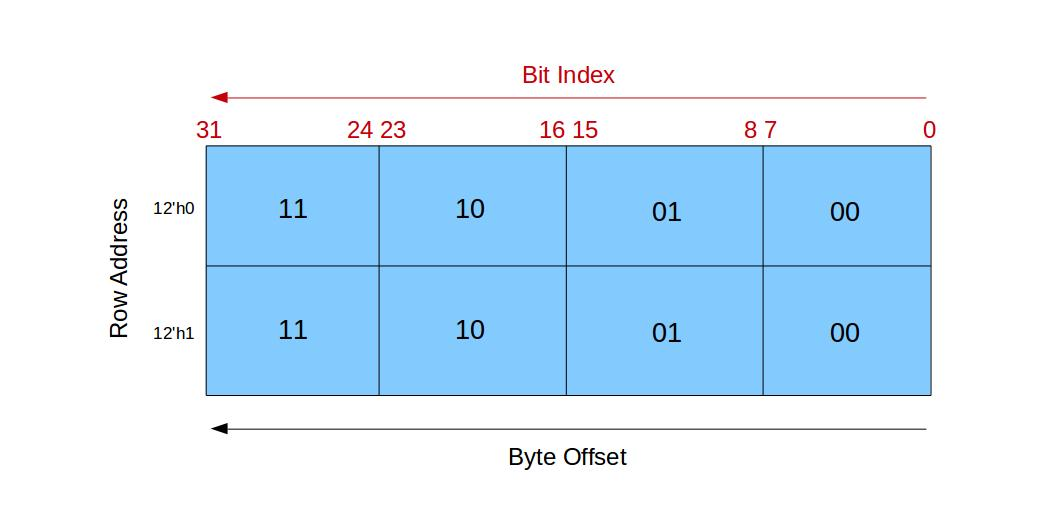
\includegraphics[width=0.6\textwidth]{endianness_img}
    \caption{Block RAM organization. The labels for row address \textbf{should read 14'h0 and 14'h1.}}
    \label{fig:endianness_img}
  \end{center}
\end{figure}

Figure \ref{fig:endianness_img} illustrates the 14-bit word addresses and the two bit byte offsets.
Observe that the RAM organization is \textbf{little-endian}, i.e. the most significant byte is at the most significant memory address (offset '11').

\subsubsection{Reading from RAMs}
Since the RAMs have 32-bit rows, you can only read data out of the RAM 32-bits at a time.
This is an issue when executing an \verb|lh| or \verb|lb| instruction, as there is no way to indicate which 8 or 16 of the 32 bits you want to read out.

Therefore, you will have to shift and mask the output of the RAM to select the appropriate portion of the 32-bits you read out.
For example, if you want to execute a \verb|lbu| on an address ending in \verb|2'b10|, you will only want bits \verb|[23:16]| of the 32 bits that you read out of the RAM (thus storing \verb|{24'b0, output[23:16]}| to a register).

\subsubsection{Writing to RAMs}
To take care of \verb|sb| and \verb|sh|, note that the \verb|we| input to the instruction and data memories is 4 bits wide.
These 4 bits are a byte mask telling the RAM which of the 4 bytes to actually write to.
If \verb|we|=\{4'b1111\}, then all 32 bits passed into the RAM would be written to the address given.

Here's an example of storing a single byte:
\begin{itemize}
  \item Write the byte \verb|0xa4| to address \verb|0x10000002| (byte offset = 2)
  \item Set \verb|we = {4'b0100}|
  \item Set \verb|dina = {32'hxx_a4_xx_xx}| (\verb|x| means don't care)
\end{itemize}

\subsection{Memory Architecture}
The standard RISC pipeline is usually depicted with separate instruction and data memories.
Although this is an intuitive representation, it does not let us modify instruction memory to run new programs.
Your CPU, by the end of this checkpoint, will be able to receive compiled RISC-V binaries though the UART, store them into instruction memory, then jump to the downloaded program.
To facilitate this, we will adopt a modified memory architecture shown in Figure \ref{fig:mem_arch}:

\textbf{TODO: replace this diagram}
\begin{figure}[hbt]
  \begin{center}
    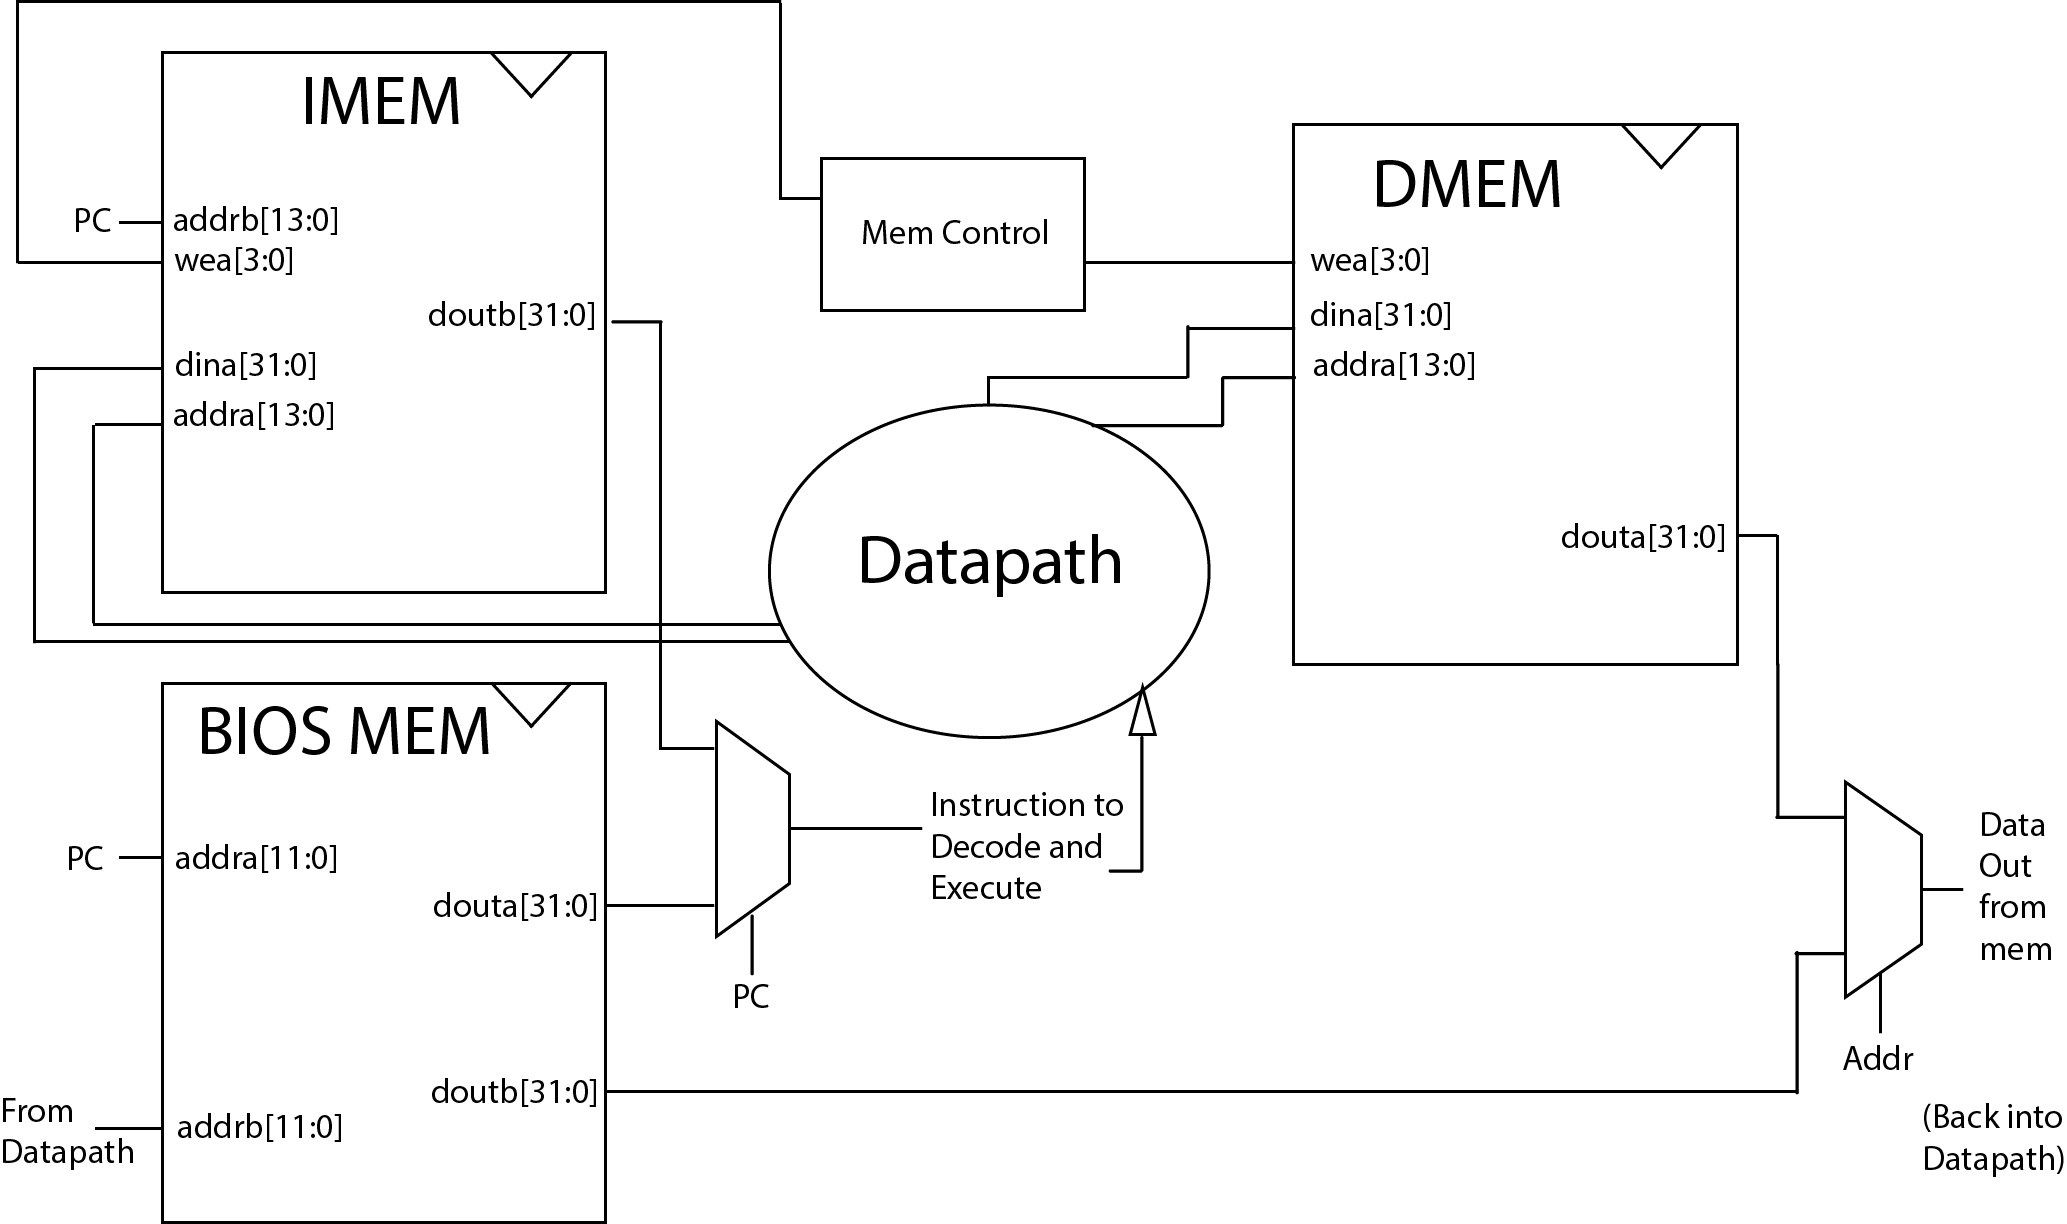
\includegraphics[width=6in]{RISCMemoryArchitectureBigMemLarge}
    \caption{Memory Architecture}
    \label{fig:mem_arch}
  \end{center}
\end{figure}

\subsubsection{Summary of Memory Access Patterns}
Your memory architecture will consist of three RAMs.
The RAMs are memory resources contained within the FPGA chip, and no external (off-chip, DRAM) memory will be used for this project.
There are RAMs for the instruction, data, and the BIOS memory.

Your processor will begin execution from the BIOS memory, which will be initialized with the BIOS program (in \verb|software/bios151v3|).
The BIOS program will be able to read from the BIOS memory (to fetch static data and instructions), and to read and write to and from instruction and data memory.
This allows the BIOS program to receive user programs over the UART from your computer and load them into instruction memory.
You can then instruct the BIOS program to jump to an instruction memory address, which begin execution of the program that you loaded.
At any time, you can press the reset button on the board to return your processor to the BIOS program.

\subsubsection{Unaligned Memory Accesses}
In the official RISC-V specification, unaligned loads and stores are supported.
However, in your project, you can ignore instructions that request an unaligned access.
The compiler will never generate unaligned accesses.

\subsubsection{Address Space Partitioning}
Your CPU will need to be able to access multiple sources for data as well as control the destination of store instructions.
In order to do this, we will partition the 32-bit address space into four regions: data memory read and writes, instruction memory writes, BIOS memory reads, and memory-mapped I/O.
This will be encoded in the top nibble (4 bits) of the memory address generated in load and store operations, as shown in Table \ref{mem_space1}.
In other words, the target memory/device of a load or store instruction is dependent on the address.
For this checkpoint, the reset signal should reset the PC to the start of BIOS memory (\verb|0x40000000|).

\begin{table}[hbt]
  \begin{center}
    \caption{Memory Address Partitions}
    \label{mem_space1}
    \begin{tabular}{l l l l l}
      \bottomrule
      \textbf{Address[31:28]} & \textbf{Address Type} & \textbf{Device} & \textbf{Access} & \textbf{Notes} \\
      \midrule
      4'b00x1 & Data & Data Memory & Read/Write &\\ %Why do we allow the 2nd bit to be x??  This can cause a conflixt with the instruction memory write.  I suppose PC[30] sets the mode?
      4'b0001 & PC  &  Instruction Memory & Read-only &\\
      4'b001x & Data & Instruction Memory & Write-Only & Only if PC[30] == 1'b1\\ %change to 4'b0011 ?? this is requested below
      4'b0100 & PC  & BIOS Memory & Read-only &\\
      4'b0100 & Data & BIOS Memory & Read-only &\\
      4'b1000 & Data & I/O & Read/Write &\\
      \bottomrule
    \end{tabular}
  \end{center}
\end{table}

Each partition specified in Table \ref{mem_space1} should be enabled only based on its associated bit in the address encoding.
This allows operations to be applied to multiple devices simultaneously, which will be used to maintain memory consistency between the data and instruction memory.

For example, a store to an address beginning with \verb|0x3| will write to both the instruction memory and data memory, while storing to addresses beginning with \verb|0x2| or \verb|0x1| will write to only the instruction or data memory, respectively.
For details about the BIOS and how to run programs on your CPU, see Section~\ref{bios_info}.

Please note that a given address maybe refers to a different memory depending on which address type it is.
For example the address \verb|0x10000000| refers to the data memory when it is a data address while a program counter value of \verb|0x10000000| refers to the instruction memory.

The note in the table above (referencing PC[30]), specifies that you can only write to instruction memory if you are currently executing in BIOS memory.
This prevents programs from being self-modifying, which would drastically complicate your processor.

\subsubsection{Memory Mapped I/O}
\label{mmio}
At this stage in the project the only way to interact with your CPU is through the UART.
The UART from Lab 5 accomplishes the low-level task of sending and receiving bits from the serial lines, but you will need a way for your CPU to send and receive bytes to and from the UART.
To accomplish this, we will use memory-mapped I/O, a technique in which registers of I/O devices are assigned memory addresses.
This enables load and store instructions to access the I/O devices as if they were memory.

To determine CPI (cycles per instruction) for a given program, the I/O memory map is also used to include instruction and cycle counters.

Table~\ref{mem_map1} shows the memory map for this stage of the project.

\begin{table}[hbt]
  \begin{center}
    \caption{I/O Memory Map}
    \label{mem_map1}
    \begin{tabular}{l l l l}
      \toprule
      \textbf{Address} & \textbf{Function} & \textbf{Access} & \textbf{Data Encoding}\\
      \midrule
      \verb|32'h80000000| & UART control & Read & \verb|{30'b0, data_out_valid, data_in_ready}| \\
      \verb|32'h80000004| & UART receiver data & Read & \verb|{24'b0, data_out}| \\
      \verb|32'h80000008| & UART transmitter data & Write & \verb|{24'b0, data_in}| \\
      \midrule
      \verb|32'h80000010| & Cycle counter & Read & Clock cycles elapsed \\
      \verb|32'h80000014| & Instruction counter & Read & Number of instructions executed \\
      \verb|32'h80000018| & Reset counters to 0 & Write & N/A \\
      \bottomrule
    \end{tabular}
  \end{center}
\end{table}

You will need to determine how to translate the memory map into the proper ready-valid handshake signals for the UART.
Your UART should respond to \verb|sw, sh, and sb| for the transmitter data address, and should also respond to \verb|lw, lh, lb, lhu, and lbu| for the receiver data and control addresses.

You should treat I/O such as the UART just as you would treat the data memory.
This means that you should assert the equivalent write enable (i.e. valid) and data signals at the end of the execute stage, and read in data during the memory stage.
The CPU itself should not check the \verb|data_out_valid| and \verb|data_in_ready| signals; this check is handled in software.
The CPU needs to drive \verb|data_out_ready| and \verb|data_in_valid| correctly.

The cycle counter should be incremented every cycle, and the instruction counter should be incremented for every instruction that is committed (you should not count bubbles injected into the pipeline or instructions run during a branch mispredict).
From these counts, the CPI of the processor can be determined for a given benchmark program.

\subsection{Testing}
\label{testing}
The design specified for this project is a complex system and debugging can be very difficult without tests that increase visibility of certain areas of the design.
In assigning partial credit at the end for incomplete projects, we will look at testing as an indicator of progress.
A reasonable order in which to complete your testing is as follows:

\begin{enumerate}
  \item Test that your modules work in isolation via Verilog testbenches
  \item Test the entire CPU one instruction at a time with hand-written assembly --- see \verb|assembly_testbench.v|
  \item Run the \verb|riscv-tests| ISA test suite
  \item Test the CPU's memory mapped I/O --- see \verb|echo_testbench.v|
\end{enumerate}

\subsubsection{Integration Testing}
Once you are confident that the individual components of your processor are working in isolation, you will want to test the entire processor as a whole. The easiest way to do this is to write an assembly program that tests all of the instructions in your ISA. A skeleton is provided for you in \verb|software/assembly_tests|. See Section \ref{assembly_tests} for details.

Once you have verified that all the instructions in the ISA are working correctly, you may also want to verify that the memory mapped I/O and instruction/data memory reading/writing work with a similar assembly program.

\subsection{Software Toolchain - Writing RISC-V Programs}
\label{toolchain}
A GCC RISC-V toolchain has been built and installed in the eecs151 home directory; these binaries will run on any of the c125m machines in the 125 Cory lab. The most relevant pieces of the toolchain are given below:
\begin{itemize}
    \item \verb|riscv64-unknown-elf-gcc|: gcc for RISC-V, compiles C code to RISC-V binaries.
    \item \verb|riscv64-unknown-elf-as|: RISC-V assembler, compiles assembly code to RISC-V binaries.
    \item \verb|riscv64-unknown-elf-objdump|: Dumps RISC-V binaries as readable assembly code.
\end{itemize}

Look at the \verb|software/c_example| folder for an example of a C program.

There are several files:
\begin{itemize}
    \item \verb|start.s|: This is an assembly file that contains the start of the program.
      It initialises the stack pointer then jumps to the \verb|main| label.
      Edit this file to move the top of the stack.
      Typically your stack pointer is set to the top of the data memory address space, so that the stack has enough room to grow downwards.

    \item \verb|c_example.ld|: This linker script sets the base address of the program.
      For checkpoint 2, this address should be in the format \verb|0x1000xxxx|
      The .text segment offset is typically set to the base of the instruction memory address space.

    \item \verb|c_example.elf|: Binary produced after running \verb|make|.\\Use \verb|riscv64-unknown-elf-objdump -D c_example.elf| to view the assembly code.
    \item \verb|c_example.asmdump|: Assembly dump of the binary.
\end{itemize}

\subsection{Assembly Tests}
\label{assembly_tests}
Hand written assembly tests are in \verb|software/assembly_tests/start.s| and the corresponding testbench is in \verb|hardware/sim/assembly_testbench.v|.

\verb|start.s| contains assembly that's compiled and loaded into the BIOS RAM by the testbench.
\begin{minted}[breaklines]{asm}
_start:

# Test ADD
li x10, 100         # Load argument 1 (rs1)
li x11, 200         # Load argument 2 (rs2)
add x1, x10, x11    # Execute the instruction being tested
li x20, 1           # Set the flag register to stop execution and inspect the result register
                    # Now we check that x1 contains 300 in the testbench

Done: j Done
\end{minted}

The \verb|assembly_testbench| toggles the clock one cycle at time and waits for register \verb|x20| to be written with a particular value (in the above example: 1).
Once \verb|x20| contains 1, the testbench inspects the value in \verb|x1| and checks it is 300, which indicates your processor correctly executed the add instruction.

If the testbench timed out it means \verb|x20| never became 1, so the processor got stuck somewhere or \verb|x20| was written with another value.

\subsection{BIOS and Programming your CPU}
\label{bios_info}

We have provided a BIOS program in \verb|software/bios151v3| that allows you to interact with your CPU and download other programs over UART.
The BIOS is basically just an infinite loop that reads from the UART, checks if the input string matches a known control sequence, and then performs the action.
%For more detailed information on the BIOS, check out this \href{http://www-inst.eecs.berkeley.edu/~cs150/fa12/project/BIOSInfo.pdf}{supplement}.
\textbf{TODO: attach BIOS document in the appendix of this spec}

To run the BIOS:
\begin{enumerate}
  \item Verify that the stack pointer and .text segment offset are set properly in \verb|start.s| and \verb|bios151v3.ld|
  \item Compile the program with \verb|make| in the \verb|software/bios151v3| directory
  \item Verify the \verb|{imem, dmem, bios_mem.v}| modules are initialized with the BIOS hex file
  \item Build a bitstream and program the FPGA
  \item Use screen to access the serial port:
    \begin{minted}[tabsize=2]{bash}
    screen $SERIALTTY 115200
    \end{minted}
  \item Press the reset button to make the CPU PC go to the start of BIOS memory
\end{enumerate}

Close screen using \verb|Ctrl-a Shift-k|, or other students won't be able to use the serial port!
If you can't access the serial port you can run \verb|killscreen| to kill all screen sessions.

If all goes well, you should see a \verb|151 >| prompt after pressing return. The following commands are available:
\begin{itemize}
    \item \verb|jal <address>|: Jump to address (hex).
    \item \verb|sw, sb, sh <data> <address>|: Store data (hex) to address (hex).
    \item \verb|lw, lbu, lhu <address>|: Prints the data at the address (hex).
\end{itemize}

As an example, running \verb|sw cafef00d 10000000| should write to the data memory and running \verb|lw 10000000| should print the output \verb|10000000: cafef00d|.
Please also pay attention that writes to the instruction memory (\verb|sw ffffffff 20000000|) do not write to the data memory, i.e. \verb|lw 10000000| still should yield \verb|cafef00d|.

In addition to the command interface, the BIOS allows you to load programs to the CPU. \textit{With screen closed}, run:
\begin{minted}[tabsize=2]{bash}
    coe_to_serial <coe_file> <address>
\end{minted}

This stores the \verb|.coe| file at the specified hex address.
In order to write into both the data and instruction memories, \textbf{remember to set the top nibble to 0x3} (i.e. \verb|coe_to_serial echo.coe 30000000|, assuming the \verb|.ld| file sets the base address to 0x10000000).
You also need to ensure that the stack and base address are set properly (See Section \ref{toolchain}).

For example, before making the \verb|mmult| program you should have set the set the base address to \verb|0x10006000| (see \ref{mmult}). Therefore, when loading the \verb|mmult| program to the FPGA you should place it into the memory that it starts aligned with the base address: \verb|coe_to_serial mmult.coe 30006000|. Then, you can start in in your screen session by using \verb|jal 10006000|.

\subsection{Target Clock Frequency}
By default, the minimum clock period is set at 50MHz.
It should be easy to meet timing at 50 MHz.
Look at the reports in \verb|hardware/build/synth/post_synth_timing_summary.rpt| and \verb|impl/post_route_timing_summary.rpt| to see if timing is met.
If you failed, the timing reports specify the critical path so you can attempt to optimize.

For this checkpoint, we will allow you to demonstrate the CPU working at 50 MHz, but for the final checkoff at the end of the semester, you will need to optimize for a higher clock speed ($\geq$ 100MHz) for full credit.
Details on how to build your FPGA design with a different clock frequency will come later.

\subsection{Matrix Multiply}
\label{mmult}
To check the correctness and performance of your processor we have provided a benchmark in \verb|software/mmult/| which performs matrix multiplication.
You should be able to load it into your processor in the same way as loading the echo program.
This program computes $S=AB$, where $A$ and $B$ are 64$\times$64 matrices. The program will print a checksum and the counters discussed in Section ~\ref{mmio}.
The correct checksum is \verb|0001f800|.
If you do not get this, there is likely a problem in your CPU with one of the instructions that is used by the BIOS but not mmult.

The matrix multiply program requires that the stack pointer and the offset of the .text segment be set properly, otherwise the program will not execute properly.

The stack pointer (set in \verb|start.s|) needs to accommodate three 64$\times$64 matrices as well as additional space for temporary results. It should be set to \verb|0x10006000| and grows downwards.

The .text segment offset (set in \verb|mmult.ld|) needs to accommodate the full set of instructions and static data in the mmult binary. It should be set to \verb|0x10006000| and.

The program will also output the values of your instruction and cycle counters (in hex).
These can be used to calculate the CPI for this program.
Your target CPI should be under 1.2, and ideally should be under 1.15.
If your CPI exceeds this value, you will need to modify your datapath and pipeline to reduce the number of bubbles inserted for resolving control hazards (since they are the only source of extra latency in our processor).
This might involve performing naive branch prediction or moving the jalr address calculation to an earlier stage.

\subsection{How to Survive This Checkpoint}
The key to this checkpoint will be to start early and work on your design incrementally. This project is not something that can be done with an all nighter and we can almost guarantee that you will not finish if you start two or three days before the due date. The key to this checkpoint will be to draw up a very detailed and organised block diagram and thoroughly understand all parts of the specification. Groups that have been successful in the past usually have unit test cases that thoroughly test every module and progressively larger integration tests. We recommend for your final integration test of the whole system that you write individual programs that thoroughly test the behavior of each instruction. The final BIOS program that you will be required to run is several 1000 lines of assembly and will be nearly impossible to use for debugging by just looking at the Modelsim waveforms.

We also encourage groups to work together and bounce ideas off of each other. The most valuable asset for this checkpoint will not be your GSIs but will be your fellow peers who you can compare notes with and discuss design aspects with in detail. However, do NOT under any circumstances share source code. We highly recommend getting adequate sleep during the weeks of this checkpoint. We realise there are not windows or clocks in the lab so it’s very easy to get carried away and work into the early morning in the lab. If you find yourself spinning your wheels, it’s probably time to go home and sleep a bit before trying again.

\subsection{How To Get Started}
It might seem overwhelming to implement all the functionality that your processor must support. The best way to implement your processor is in small increments, checking the correctness of your processor at each step along the way. Here is a guide that should help you plan out checkpoint 1:

\begin{enumerate}
  \item \textbf{Design.} You should start with a comprehensive and detailed design/schematic. We suggest that you think carefully about all the functionality and instructions your processor needs to support and enumerate all the control signals that you will need. Be especially careful when designing the memory fetch stage of your pipeline as all the memories we use (BIOS, inst, data, IO) are synchronous.
  \item \textbf{First steps.} You should get started by implementing some modules that are straightforward to write and test. We suggest you get started by writing \verb|RegFile.v|, for which there has been a template provided in the project skeleton. Once you finish writing the regfile, test it comprehensively by writing a Verilog testbench. Look at the Register File section for details on what the test should verify.
  \item \textbf{Control Unit + other small modules.} Next try implementing your control unit, the ALU, and any other small independent modules that you identified in your design. Make sure you unit test these aggressively, so that you verify their correctness and get used to writing Verilog testbenches.
  \item \textbf{Memory.} Create your memory controller and other auxiliary structures. Only add the BIOS memory in the instruction fetch stage and only add the data memory block RAM in the memory stage of your pipeline. This will keep things simple in order to test the base functionality of your processor.
  \item \textbf{Connect stages and pipeline.} Now you should have all of the modules ready to connect them together and pipeline them by inserting registers between the stages. At this point, you should be able to run integration tests using assembly tests for most R and I type instructions.
  \item \textbf{Implement handling of control hazards.} Now insert bubbles into your pipeline to resolve control hazards associated with JAL, JALR, and branch instructions. Don't worry about data hazard handling for now. Test that your control instructions work properly with assembly tests. You can insert explicit NOP instructions in your tests to get around data dependencies.
  \item \textbf{Implement data forwarding for data hazards.} Add forwarding muxes to the proper place in your datapath and forward the outputs of the ALU and memory stage. Implement a hazard unit that can detect data dependencies and set the control signals for the forwarding muxes accordingly. Remember that you might have to forward to ALU input A, ALU input B, and data to write to memory. Test forwarding aggressively; most of your bugs will come from incomplete or faulty forwarding logic. Make sure you test forwarding from memory and from the ALU, and with control instructions.
  \item \textbf{Add BIOS memory reads.} Add the BIOS memory block RAM to the memory stage to be able to load data from the BIOS memory. Write assembly tests that contain some static data stored in the BIOS memory and verify that you can read that data.
  \item \textbf{Add Inst memory writes and reads.} Add the instruction memory block RAM to the memory stage to be able to write data to it when executing inside the BIOS memory. Also add the instruction memory block RAM to the instruction fetch stage to be able to read instructions from the inst memory. It is crucial to write tests to stress this portion of the processor; we suggest writing tests that first write instructions to the instruction memory, and then jump (using jalr) to instruction memory to see the right instructions are executed.
  \item \textbf{Add cycle counters.} Begin to add the memory mapped IO components, by first adding the cycle and instruction counters. These are just 2 32-bit registers that your CPU should update on every cycle and every instruction respectively. Write tests to verify that your counters can be reset with a SW instruction, and can be read from using a LW instruction.
  \item \textbf{Integrate UART.} Add the UART to the memory stage, in parallel with the data, instruction, and BIOS memories. Detect when an instruction is accessing the UART and route the data to the UART accordingly. Make sure that you are setting the UART ready/valid control signals properly as you are feeding or retrieving data from it. This part can be tricky, ask a TA for a full explanation of how a program would communicate with the UART. We have provided you with the \verb|echo_testbench| which performs a test of the UART. You should extend this testbench with more comprehensive tests, as many bugs can be traced to a faulty UART integration.
  \item \textbf{Run the BIOS.} If everything so far has gone well, you can try making the CPU with instantiating the BIOS memory with the BIOS program. Impact the CPU on the board and verify that the BIOS performs as expected. As a precursor to this step, you might try to make the CPU with instantiating the BIOS memory with the echo program, since it is a smaller and easier to analyze program.
  \item \textbf{Run matrix multiply.} As a final step to check your implementation, you should be able to load the \verb|mmult| program with the \verb|coe_to_serial| utility, and run \verb|mmult| on the FPGA. Verify that it returns the correct checksum.
  \item \textbf{Check CPI.} Now that your processor is complete as far as functionality goes, compute the CPI when running the \verb|mmult| program. If you achieve a CPI below 1.2, that is acceptable, but if your CPI is larger than that, you should think of ways to reduce it. With this step complete, you are ready for the next checkpoint.
\end{enumerate}

\subsection{Checkoff}

The checkoff for this specification is divided into two stages: block diagram/design and implementation. The second part will require significantly more time and effort than the first one. As such, completing the block diagram in time for the design review is crucial to your success in this project.

\subsubsection{\blockDiagramTaskName: Block Diagram}
The first checkpoint requires a detailed block diagram of your datapath. The diagram should have a greater level of detail than a high level RISC datapath diagram. You may complete this electronically or by hand. If working by hand, we recommend working in pencil and combining several sheets of paper for a larger workspace. You should also be able to describe in detail any smaller sub-blocks in your diagram. If working electronically, you can use a schematic capture program, Logisim, or anything that can produce a diagram that is easily modifiable. Though the textbook diagrams are a decent starting place, please remember that they use asynchronous-read memories for the instruction and data memories, and we will be using synchronous-read block RAMs. Additionally, at this point we recommend that you have a completely functional UART, ALU, ALU decoder, and register file modules (see \ref{reg_file}), though we will not be checking this.

\textbf{\blockDiagramTaskName \space is due in lab no later than \blockDiagramDueDate}. You are required to go over your design with a GSI during lab. Be prepared to talk generally about how you came up with your design and defend your design decisions.

\subsubsection{Non-Checkpoint Weeks}

In labs, you probably found that you spent significantly more time debugging and verifying your design than actually writing Verilog. Though your skills are continually improving, this project involves a complex system and as such, bugs are inevitable. Design verification can take more than twice as long as writing the initial implementation. Given this, we recommend that you have completed your first stab at writing the Verilog and associated module testbenches for your processor by the end of this week.

\subsubsection{\baseCPUTaskName: Base RISCV151 System}
This checkpoint requires a fully functioning three stage RISC-V CPU as described in this specification. Checkoff will consist of a demonstration of the BIOS functionality, storing a program (echo and mmult) over the serial interface, and successfully jumping to and executing the program.

\textbf{\baseCPUTaskName \space materials should be committed to your project repository by \baseCPUDueDate.}

\subsubsection{Checkpoints 1 \& 2 Deliverables Summary}
\begin{center}
  \begin{tabular}{m{30mm} m{35mm} m{70mm}}
    \toprule
    \textbf{Deliverable} & \textbf{Due Date} & \textbf{Description} \\
    \midrule
    Block Diagram & \blockDiagramDueDate & Sit down with a GSI and go over your design in detail\\
    \midrule
    RISC-V CPU & \baseCPUDueDate \linebreak Check in code to Github & Demonstrate that the BIOS works, you can use \verb|coe_to_serial| to load the echo program, \verb|jal| to it from the BIOS, and have that program successfully execute. Load the mmult program with \verb|coe_to_serial|, \verb|jal| to it, and have it execute successfully and return the benchmarking results and correct checksum. Your CPI should be under 1.2\\
    \bottomrule
  \end{tabular}
\end{center}

\pagebreak

\section{Checkpoint 3 - I/O, FIFO, HDMI, Line Accelerator}
In checkpoint 3 of this project you will implement a memory mapped I/O interface to user inputs and outputs (push buttons, LEDs, and switches). To buffer user inputs to your processor you will integrate the FIFO built in lab.

You will also implement (part of) an HDMI controller with a frame buffer that can be written to by both your CPU and a line-drawing accelerator. You will implement the line-drawing accelerator to take arguments from your CPU and fill in the frame buffer for you, with lines. At first you will use a block RAM frame buffer. As an extension, you will use the Pynq-Z1's DRAM to support full 8-bit colour output.

\subsection{User I/O Interfacing}
In lab, you built a synchroniser, debouncer and an edge detector that were used to take in various user inputs (push buttons mostly). Now, we want our processor to have access to these inputs (and the switches) and also to be able to drive outputs such as the LEDs. We will extend our memory map to give user programs access to these I/Os.

When a user pushes a button on the Pynq-Z1 board, the button's signal travels through the synchroniser $\rightarrow$ debouncer $\rightarrow$ edge detector chain. The result is a single clock cycle wide pulse coming out of the edge detector that represents a single button press. If we just extended our memory map to directly include the outputs from the edge detector, the processor would have to read from those locations on every clock cycle to be sure it didn't miss any user inputs.

(We will sometimes refer to these devices as GPIO, meaning General-Purpose I/O.)

This is clearly not feasible as it would starve our processor. We need a way to buffer user inputs and let the processor consume them when it has time to do so. This buffer will be implemented as a FIFO.

\subsubsection{Hookup FIFO to User I/O}
We'll use the FIFO to buffer user I/O signals for the RISC-V core to consume via memory-mapped I/O. We want to give the processor access to these I/Os:

\begin{itemize}
  \item Switches
  \item GPIO LEDs (the ones on the Pynq-Z1 board)
  \item Push-buttons
  \item PMOD LEDs

\textbf{Note:} You won't be able to use the PMOD LEDs at the same time as the USB UART and the I2S controller, owing to a lack of PMOD ports on the Pynq-Z1. You can thus omit the \verb|PMOD_LEDS| signal from the memory connection; it's left in for illustrative purposes.

\end{itemize}

Here is the new memory map:
\begin{table}[hbt]
  \begin{center}
    \caption{Updated Memory Map with User I/O}
    \label{mem_map2}
    \begin{tabular}{l l l l}
      \toprule
      \textbf{Address} & \textbf{Function} & \textbf{Access} & \textbf{Data Encoding}\\
      \midrule
      32'h80000000 & UART control & Read & \{30'b0, DataOutValid, DataInReady\} \\
      32'h80000004 & UART receiver data & Read & \{24'b0, DataOut\} \\
      32'h80000008 & UART transmitter data & Write & \{24'b0, DataIn\} \\
      \midrule
      32'h80000010 & Cycle counter & Read & Total number of cycles \\
      32'h80000014 & Instruction counter & Read & Number of instructions executed \\
      32'h80000018 & Reset counters to 0 & Write & N/A \\
      \midrule
      32'h80000020 & GPIO FIFO Empty & Read & \{31'b0, empty\} \\
      32'h80000024 & GPIO FIFO Read Data & Read & \{28'b0, BUTTONS[3:0] \} \\
      \midrule
      32'h80000028 & Switches & Read & \{30'b0, SWITCHES[1:0]\} \\
      \midrule
      32'h80000030 & GPIO LEDs \& PMOD LEDs & Write & \{16'b0, PMOD\_LEDS[7:0], 2'b0, LEDS[5:0]\} \\
      \midrule
    \end{tabular}
  \end{center}
\end{table}

We want to use our FIFO for the signals enumerated in the GPIO FIFO Read Data row. On any given clock cycle, when any of the button signals pulse high, the FIFO should be written to with the status of all the button signals. The CPU should be able to read the empty signal of the FIFO, and it should be able to read out data from the FIFO with the FIFO's \verb|rd_en| signal controlled by your memory logic.

Modify \verb|z1top.v| and \verb|Riscv151.v| by instantiating your FIFO, hooking up its ports to the user I/O signals, and connecting your FIFO's read interface to the RISC-V core.

\subsubsection{User I/O Test Program}
We have provided a program that you can use to test your FIFO and memory map. It is found in \verb|software/user_io_test|. To run it, synthesize, implement and program your FPGA design as usual. Then, reset your design. Run \verb|make| in the \verb|user_io_test| folder, and then run \verb|coe_to_serial user_io_test.coe 30006000|. Then \verb|screen| and \verb|jal 10006000| from the BIOS to jump into the user I/O test program.

This program has several commands to help you debug and verify functionality:
\begin{itemize}
  \item \verb|read_buttons| - This command will have the CPU read from the GPIO FIFO until it is empty, decode the button press data, and print it out.
  \item \verb|read_switches| - This command will have the CPU read the slide switches' address and will print out the state of the switches.
  \item \verb|led <data>| - This command will write the \verb|<data>| (32-bits in hex) that you specify to the GPIO LEDs address. Keep in mind we only have 6 LEDs on the board (unless you use the LED PMOD), so you only write values up to 0x3F.
  \item \verb|exit| - Jump back into BIOS.
\end{itemize}

Once you are confident that all the user I/Os are working, move on to the next section.

\subsection{Checkpoint 3 Deliverables Summary}

\begin{center}
  \begin{tabular}{m{30mm} m{35mm} m{70mm}}
    \toprule
    \textbf{Deliverable} & \textbf{Due Date} & \textbf{Description} \\
    \midrule
    User I/O + FIFOs + HDMI video controller + line drawing accelerator & \audioDueDate & Demonstrate the working user IO test program. Explain your testing methodology for the FIFOs and any system level integration testbenches you created.  Demonstrate a working static image test. Demonstrate line or image drawing from both the CPU and the accelerator. \\
    %Demonstrate the \itwos{} visual piano
    \bottomrule
  \end{tabular}
\end{center}

\pagebreak

\section{Final Checkpoint - Optimization}

This optimization checkpoint is lumped with the final checkpoint and the checkoff will occur at the same time. This part of the project is designed to give students freedom to implement the optimizations of their choosing to improve the performance of their processor.

The general optimization goal for this project is to achieve maximal performance on the \verb|mmult| program, as defined by the 'Iron Law' of Processor Performance.

\begin{equation*}
\frac{\text{Time}}{\text{Program}} = \frac{\text{Instructions}}{\text{Program}} \times \frac{\text{Cycles}}{\text{Instruction}} \times \frac{\text{Time}}{\text{Cycle}}
\end{equation*}

Your goal is to minimize the execution time of \verb|mmult|. The number of instructions is fixed, but you have freedom to change the CPI and the CPU clock frequency. Often you will find that you will have to sacrifice CPI to achieve a higher clock frequency, but there also will exist opportunities to improve one or both of the variables without compromises.

\subsection{Clock Generation Info + Changing Clock Frequency}
Open up \verb|z1top.v|. You will notice a top level input called \verb|USER_CLK|. This signal comes from a crystal on the ML505 board and it comes into our FPGA design. It is a 125 MHz clock signal, which we will use to derive our CPU clock.

Scrolling down a little further, you will see an instantiation of \verb|PLLE2_ADV|, which is a PLL (phase locked loop) primitive on the FPGA. This is a circuit that lets us create a new clock from a known clock with a user-specified multiply-divide ratio.

The \verb|CLKIN| input clock of the PLL. is driven by the 125 MHz \verb|user_clk_g| (buffered \verb|USER_CLK|). The PLL divides this frequency by the \verb|DIVCLK_DIVIDE| parameter, which is set to 5. Thus, internally, the PLL creates a 25 MHz clock. Then, this multiplied clock is divided by \verb|CLKFBOUT_MULT| parameter and divided by the \verb|CLKOUT0_DIVIDE| parameter. In our case, this yields \verb|125_000_000 / 5 * | \newline \verb|34 / 17 = 50_000_000|, our desired CPU clock. Finally, the multiplied and divided clock shows up at the \verb|CLKOUT0| output clock of the PLL, which is connected to \verb|cpu_clk|. The \verb|cpu_clk| is buffered and \verb|cpu_clk_g| is used in our CPU and other modules.

Play around with the multipliers and divisors in the PLL to generate a faster (or slower) clock. You may have to consult Xilinx's documentation on the \verb|PLL2E_ADV| primitive. (You can also use the Clocking Wizard IP generator in Vivado to generate this instantiation.) The parameters can't be set arbitrarily and there are a few caveats. The multipliers and divisors must be integers and you must fall within the device's operating frequency range - Vivado will complain if you don't. A few frequencies to try are: 60 MHz, 75 MHz, and 100 MHz.

\subsection{Critical Path Identification}
Begin by pulling the latest skeleton files from the staff repository: \verb|git pull staff master|. After running synthesis and implementation, your FPGA design will be placed and routed, and timing analysis will be performed to determine the critical path(s) of your design. The timing tools will automatically figure out the CPU clock timing constraint based on the multiply-divide ratio you used in your PLL.

You can find the critical path in the timing reports from your implementation step (in the Flow Navigator). Expand \emph{Implemented Design} $\rightarrow$ Select \emph{Report Timing Summary}. You are interested in the timing paths for \verb|cpu_clk_g| which is the clock used by your CPU and the rest of your design.

What is your critical path?

For each timing path look for the attribute called ``slack''. Slack describes how much extra time the combinational delay of the path has before the rising edge of the receiving clock. It is a setup time attribute. Positive slack means that this timing path resolves and settles before the rising edge of the clock, and negative slack indicates a setup time violation.

You will then see the source and destination of the path which you can usually map to a net in your design. You can also see (And even visualise) the actual logic path that starts at the source and follows some logic in your design until it gets to the destination.

There are 3 common delay types that you will encounter during optimization. Most of the \verb|Trc*| delays are RAM delays that represent either Clk-to-q delays or setup time constraints. \verb|Tilo| delays are combinational delays through LUTs. \verb|net| delays are routing delays. If you want details on a specific delay type, check the \href{https://www.xilinx.com/support/documentation/data_sheets/ds202.pdf}{Virtex 5 Datasheet} starting from page 40.

\verb|net| delays include a fanout attribute. You will likely want to minimize fanout of a given net along a timing path in order to reduce routing delay. You will notice that as a percentage of total delay, routing dominates over combinational logic delay. As you continue optimization, you can reach the point where the routing delay percentage of total delay will be roughly one-half.

\subsubsection{Finding Actual Critical Paths}
When you first check the timing report with a 50 MHz clock, you might not see your 'actual' critical path. 50 MHz is an easy timing constraint for the tools to meet for most CPU designs and thus, the tools will only attempt to optimize routing until timing is met, and will then stop. The critical paths you see in the report may not be the 'actual' critical paths since the tools haven't been pushed to the limit.

We recommend that you begin optimization by increasing the clock frequency slowly and re-running synthesis and implementation until the routing tool fails to meet timing. At this point, you know that the tools tried as hard as they could and just missed timing, so then the critical paths you see in the report are the 'actual' ones you need to work on.

As an aside, don't try to increase the clock speed up all the way to 100 MHz initially, since that will cause the routing tool to give up even before it tried anything. Thus, you will get 'false' critical paths, that aren't necessarily where you should spend your time when optimizing.

\subsection{Optimization Tips}
As you work on achieving a higher clock speed, you will likely notice that the routing tool (PAR) is quite temperamental. You may find that your design might meet timing for a given clock speed, but after making a small, insignificant design change, the tool fails to meet timing. This is because PAR uses a random seed as a starting point in its algorithm. Sometimes it is a 'good' seed and yields an optimal result, but a small design change may cause the same seed to become 'bad' for that design and it yields a sub-optimal result.

As you optimize your design, you will want to try running \verb|mmult| on your newly optimized designs as you go along. You don't want to make a lot of changes to your processor, get a better clock speed, and then find out you broke something along the way.

You will find that sacrificing CPI for a better clock speed is a good bet to make in some cases, but will worsen performance in others. You should keep a record of all the different optimizations you tried and the effect they had on CPI and minimum clock period; this will be useful for the final report when you have to justify your optimization and architecture decisions.

There is no limit to what you can do in this section. The only restriction is that you have to run the original, unmodified \verb|mmult| program so that the number of instructions remain fixed. You can add as many pipeline stages as you want, stall as much or as little as desired, add a branch predictor, or perform any other optimizations. If you decide to do a more advanced optimization (like a 5 stage pipeline), ask the staff to see if you can use it as extra credit in addition to the optimization.

You will be graded based on the best \verb|mmult| performance you were able to achieve, as well as your documentation/reasoning for your architecture modifications in the process of optimization. You need to also take into consideration area usage when optimizing, so be sure to keep records as you optimize.

\pagebreak

\section{Optimizations, Extra Credit, and Grading}


\textbf{All groups must complete the final checkoff by \finalCheckoffDueDate.} Use the week prior to your final checkoff for code cleanup, optimizations, late checkpoints, and optional extra credit projects.

\subsection{Grading on Optimization}

To receive full credit, you must demonstrate a working CPU at an optimized clock frequency (above 50MHz) that has a working BIOS, can load and execute programs (both echo and mmult), can receive, process, and send to user I/O, and has a working \itwos{} controller. Additionally, you will be graded on total FPGA resource utilization, with the best designs using as few resources as possible. If you are unable to make the deadline for any of the checkpoints, it is still in your best interest to complete the design late, as you can still receive most of the credit if you get a working design by the final checkoff.

Credit for your area optimizations will be calculated using a cost function. At a high level, the cost function will look like:

\[\mathrm{Cost}=\mathrm{C_{LUT}} \times \mathrm{\# of LUTs} + \mathrm{C_{RAMB}} \times \mathrm{\#of RAMBs} + \mathrm{C_{REG}} \times \mathrm{\#of Slice Registers} \]

where $\mathrm{C_{LUT}}$, $\mathrm{C_{RAMB}}$, and $\mathrm{C_{REG}}$ are constant value weights that will be decided upon based on how much each resource that you use should cost. As part of your final grade we will evaluate the cost of your design based on this metric. Keep in mind that cost is only one very small component of your project grade. Correct functionality is far more important.

\subsection{Checkpoints}
\label{checkoff}

We have divided the project up into checkpoints so that you (and the staff) can pace your progress. The due dates are indicated at the end of each checkpoint section, as well as in the \textbf{Project Timeline} (Section \ref{project_timeline}) at the end of this document. During the week each checkpoint is due, you will be required to get your implementation checked off by the GSI in the lab section you are enrolled in.

\subsection{Style: Organization, Design}
\label{style}

Your code should be modular, well documented, and consistently styled. Projects with incomprehensible code will upset the graders.

\subsection{Final Project Report}

Upon completing the project, you will be required to submit a report detailing the progress of your EECS151/251A project. The report should document your final circuit at a high level, and describe the design process that led you to your implementation.  We expect you to document and justify any tradeoffs you have made throughout the semester, as well as any pitfalls and lessons learned (not make excuses for why something didn't work).  Additionally, you will document any optimizations made to your system, the system's performance in terms of area (resource use), clock period, and CPI, and other information that sets your project apart from other submissions.

The staff emphasizes the importance of the project report because it is the product you are able to take with you after completing the course.  All of your hard work should reflect in the project report. Employers may (and have) ask to examine your EECS151/251A project report during interviews. Put effort into this document and be proud of the results. You may consider the report to be your medal for surviving EECS151/251A.

\subsubsection{Report Details}
You will turn in your project report on Gradescope by the final checkoff date. The report should be around 8 pages total with around 5 pages of text and 3 pages of figures ($\pm$ a few pages on each). Ideally you should mix the text and figures together.

Here is a suggested outline and page breakdown for your report. You do not need to strictly follow this outline, it is here just to give you an idea of what we will be looking for.

\begin{itemize}
  \item \textbf{Project Functional Description and Design Requirements}. Describe the design objectives of your project.  You don't need to go into details about the RISC-V ISA, but you need to describe the high-level design parameters (pipeline structure, memory hierarchy, etc.) for this version of the RISC-V. ($\approx$ 0.5 page)
  \item \textbf{High-level organization}. How is your project broken down into pieces. Block diagram level-description. We are most interested in how you broke the CPU datapath and control
  down into submodules, since the code for the later checkpoints will be pretty consistent across all groups. Please include an updated block diagram ($\approx$ 1 page).
  \item \textbf{Detailed Description of Sub-pieces}. Describe how your circuits work. Concentrate here on novel or non-standard circuits. Also, focus your attention on the parts of the design that were not supplied to you by the teaching staff. For instance, describe the details of your \itwos{} controller, FIFOs, DVI controller, and any extra credit work. ($\approx$ 2 pages).
  \item \textbf{Status and Results}. What is working and what is not? At what frequency (50MHz or greater) does your design run? Do certain checkpoints work at a higher clock speed while others only run at 50 MHz? Please also provide the number of LUTs and SLICE registers used by your design, which can be found by running \verb|make report|. Also include the CPI and minimum clock period of running \verb|mmult| for the various optimizations you made to your processor. This section is particularly important for non-working designs (to help us assign partial credit). ($\approx$ 1-2 pages).
  \item \textbf{Conclusions}. What have you learned from this experience? How would you do it different next time? ($\approx$ 0.5 page).
  \item \textbf{Division of Labor. This section is mandatory. Each team member will turn in a separate document from this part only}. The submission for this document will also be on Gradescope. How did you organize yourselves as a team. Exactly who did what? Did both partners contribute equally? Please note your team number next to your name at the top. ($\approx$ 0.5 page).
\end{itemize}

When we grade your report, we will grade for clarity, organization, and grammar. Make sure to proofread and correct mistakes before turning it in. Submit your report to the Gradescope assignment. Only one partner needs to submit the shared report, while each individual will need to submit the division of labor report to a separate Gradescope assignment.

\subsection{Extra Credit}
\label{extra_credit}
Teams that have completed the base set of requirements are eligible to receive extra credit worth up to 10\% of the project grade by adding extra functionality and demonstrating it at the time of the final checkoff.

The following are suggested projects that may or may not be feasible in one week.
\begin{itemize}
  \item Integrating your Tone Generator and I2S Controller from the Lab Assignments (see section \ref{audio_extra_credit} for details)
  \item Branch Predictor: Implement a two bit (or more complicated) branch predictor with a branch history table (BHT) to replace the naive 'always taken' predictor used in the project
  \item 5-Stage Pipeline: Add more pipeline stages and push the clock frequency past 100MHz
  \item Audio Recording: Enable capturing mic input from the \itwos{} controller (for undergrads)
  \item RISC-V M Extension: Extend the processor with a hardware multiplier and divider
  \item 3 (or more) bit color: Increase the size of the framebuffer to have control of the RGB content of each pixel
  \item Dynamic Resolution: Allow the processor to control the output resolution of the DVI controller at runtime
\end{itemize}

When the time is right, if you are interested in implementing any of these, see the staff for more details.

\subsection{Project Grading}
\label{deadlinegrading}

\begin{description}
  \item[80\%] {Functionality} at project due date. Your design will be subjected to a comprehensive test suite and your score will reflect how many of the tests your implementation passes.
  \item[5\%] {Optimization} at project due date. This grade is a function of the resources used by your implementation. This score is contingent on implementing all the required functionality.  An incomplete project will receive a zero in this category.
  \item[5\%] {Checkpoint} functionality. You are graded on functionality for each completed checkpoint. The total of these scores makes up 5\% of your project grade. The weight of each checkpoint's score may vary.
  \item[10\%] {Final report} and {style} demonstrated throughout the project.
\end{description}

Not included in the above tabulations are point assignments for extra credit as discussed above. Extra credit is discussed below:

\begin{description}
  \item[Up to 10\%] Additional functionality. Credit based on additional functionality will be qualified on a case by case basis. Students interested in expanding the functionality of their project must meet with a GSI well ahead of time to be qualified for extra credit. Point value will be decided by the course staff on a case by case basis, and will depend on the complexity of your proposal, the creativity of your idea, and relevance to the material taught.
\end{description}

\section{Project Timeline}
\label{project_timeline}

\begin{table}[h!]
  \centering
  \begin{center}
  \begin{tabular}{l l l}
    \toprule
    {Checkpoint} &{Deliverable} & {Due Date} \\
    \midrule
    1 \& 2: RISCV151 Processor & Design Review &  \blockDiagramDueDate\\
     & In-Lab Checkoff & \baseCPUDueDate \\
    \midrule
    3: IO, FIFOs, Video/Graphics & In-Lab Checkoff &  \audioDueDate \\
     & Project Interview & \\
    \midrule
    Final Checkoff, Extra Credit, &    In-Lab Checkoff        & \finalCheckoffDueDate \\
    and Optimizations             & Github code submission    &  \\
    \midrule
    Final Report                  &   Gradescope submission     & \finalReportDueDate \\
    \bottomrule
  \end{tabular}
  \end{center}
\caption{EECS151 \currentSemester \space Project Timeline}\label{tab:master}
\end{table}

\newpage
\section{Appendix A - Tone Generator \& I2S Extra Credit}\label{audio_extra_credit}
This section details an extra credit opportunity for you to integrate your tone generator and I2S controller from the lab assignments with your RISCV processor.

\subsection{Summary}
You will add the \verb|tone_generator| created in lab to the design as a peripheral and allow programs to access its \verb|tone_switch_period| and \verb|output_enable| inputs over memory mapped I/O. You will be able use your processor to simulate the \verb|music_streamer| FSM built in lab using software only.

You will extend your \itwos{} audio controller created in lab to fetch samples from an asynchronous FIFO that the processor will write to. This will allow your processor to synthesize and send arbitrary waveforms to the \itwos{} DAC. Once you have the tone generator and I2S modules working, you will be able to load a program onto your processor which allows you to use your keyboard as a piano. The program synthesizes sine waves of various frequencies based on what key you are pressing and will transmit the wave to the codec so you can hear the music you play through your headphones.

Get started by pulling the latest skeleton files from the staff repository: \verb|git pull staff master|.

\subsection{Tone Generator Hookup}
Copy over your \verb|tone_generator.v| from Lab 5 to the \verb|hardware/src/audio/| directory. Recall that your \verb|tone_generator| takes a \verb|tone_switch_period| which describes how many clock cycles the \verb|tone_generator| takes to invert its \verb|square_wave_out| output. There is also an \verb|output_enable| input into the \verb|tone_generator| which gates the \verb|square_wave_out| output low.

We want to give our RISC-V core the ability to set the \verb|tone_switch_period| and the \verb|output_enable| of the tone generator. Here is the addition to the memory map:

\begin{table}[hbt]
  \begin{center}
    \caption{Tone Generator Memory Map Additions}
    \label{mem_map2_2}
    \begin{tabular}{l l l l}
      \toprule
      \textbf{Address} & \textbf{Function} & \textbf{Access} & \textbf{Data Encoding}\\
      \midrule
      32'h80000034 & Tone Generator Output Enable & Write & \{31'b0, output\_enable\} \\
      32'h80000038 & Tone Generator Tone Switch Period & Write & \{8'b0, tone\_switch\_period[23:0]\} \\ \bottomrule
    \end{tabular}
  \end{center}
\end{table}

Modify \verb|z1top.v| and \verb|Riscv151.v|. Instantiate the \verb|tone_generator| at the top level and connect \verb|square_wave_out| to the \verb|AUDIO_PWM| output. The \verb|output_enable| signal should be connected to the AND of \verb|BUTTONS[0]| and the register that's written by the CPU. The \verb|tone| signal should be connected to another register that's written by the CPU via memory mapped I/O.

Modify your CPU to take in and output any signals it needs for this tone generator hookup.

\subsubsection{Testing the Tone Generator}
We have provided a program to test your tone generator and its memory map. It can be found in \verb|software/tone_gen_test/|. Compile and run the program just as you did for the \verb|user_io_test|. Make sure the first slide switch is on. \verb|jal| to the program from the BIOS, and you can play with these commands:

\begin{itemize}
  \item \verb|on| - Flips the output enable register high
  \item \verb|off| - Flips low the output enable register low
  \item \verb|tone <tone_switch_period>| - Writes the user specified \verb|tone_switch_period| (32-bits in hex) to the tone switch period address
  \item \verb|exit| - Jumps back to the BIOS
\end{itemize}

Calculate the \verb|tone_switch_period| for a 440Hz tone with a 50 MHz clock and try sending the command for that through the test program. Verify that the piezo speaker is buzzing at 440Hz by comparing it to a square wave at the same frequency via a \href{http://onlinetonegenerator.com/}{tone generator}.

\subsubsection{Music Streamer in Software}
Now that we have access to user I/Os and access to the tone generator, we can fully implement the music streamer and sequencer FSM from lab 4 entirely in software!

Kind of... We still don't have enough buttons so are limited in the functionality we can implement. The workaround is to not include the sequencer from lab 4 (which was an optional part anyway). Since button 3 is now our reset, we can use buttons 0-2 to implement the rest of the functionality. The software version of the music streamer maps button 0 to play/pause, button 1 to reverse, and button 2 to tempo reset. As you'll have noticed, there is no way to change the tempo, so if you would like to add that functionality, feel free to edit the .c file. You can use the switches as we did in the lab, but keep in mind that they behave differently to the buttons. How you do this part is up to you, but it is enough to show a version with only play/pause, reverse, and tempo reset. Ask a GSI if you need help.

The music streamer program can be found in \verb|software/music_streamer|. To use this program, use the same scripts from Lab 3 to generate a music data file from a MusicXML file, and then convert that data file to a static array declaration that can be used in a C program.

\begin{minted}[frame=single]{bash}
python scripts/musicxml_parser.py musicxml/Row_Row_Row_Your_Boat.mxl music.txt
\end{minted}

You will now have a \verb|music.txt| file in the \verb|/software/music_streamer| directory with the music data. Now we use the \verb|c_array_generator.py| script to create a static array declaration using this file.

\begin{minted}[frame=single]{bash}
python scripts/c_array_generator.py music.h music.txt
\end{minted}

Now, we have a file called \verb|music.h| that has a static array declaration filled with the music data. This serves exactly the same purpose as the ROM that was generated in Lab 3.

To build the \verb|music_streamer| program and place it on your processor, execute:
\begin{minted}[frame=single]{bash}
make
coe_to_serial music_streamer.coe 3000a000
screen $SERIALTTY 115200
151> jal 1000a000
\end{minted}

The \verb|music_streamer| functions exactly like it does in Lab 3, but the state machine that was implemented directly in hardware, is now implemented in software. Here is the state machine diagram for reference:

\begin{center}
  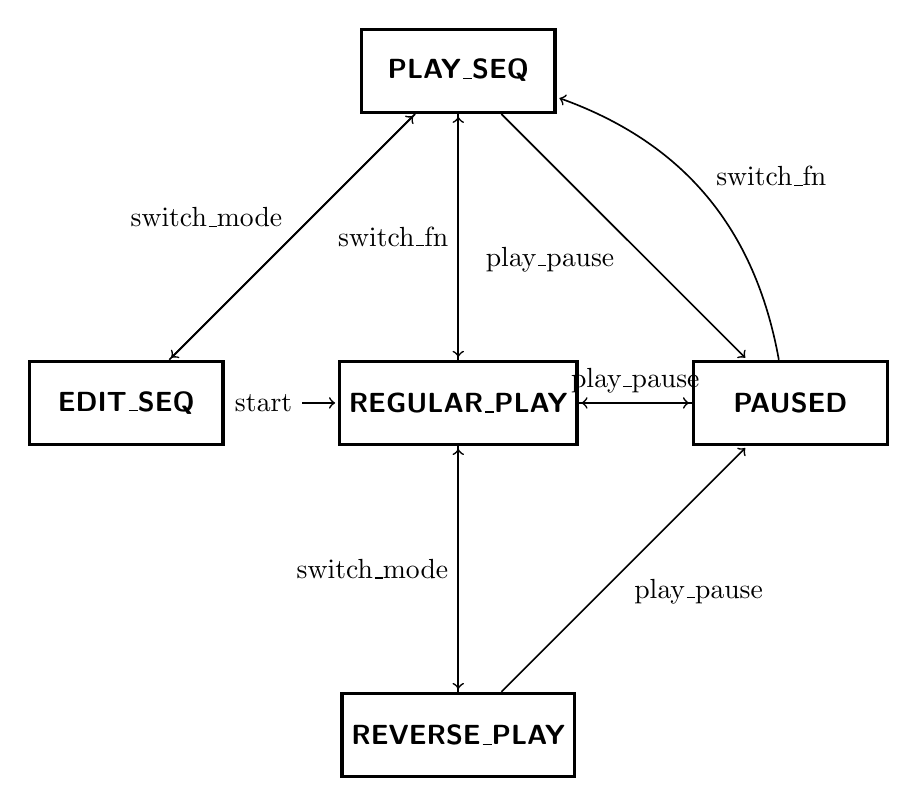
\begin{tikzpicture}[shorten >=1pt, node distance=10cm,on grid, auto, semithick]
  \tikzstyle{state} = [draw, very thick, fill=white, rectangle, minimum height=3em, minimum width=7em, node distance=12em, font={\sffamily\bfseries}]
  \tikzstyle{stateEdgePortion} = [black,thick];
  \tikzstyle{stateEdge} = [stateEdgePortion,->];
  \tikzstyle{edgeLabel} = [pos=0.5, text centered, font={\sffamily\small}];

  \node[state,initial](rp) {REGULAR\_PLAY};
  \node[state](revp) [below =of rp]{REVERSE\_PLAY};
  \node[state](p) [right=of rp]{PAUSED};
  \node[state](playseq) [above=of rp]{PLAY\_SEQ};
  \node[state](editseq) [left=of rp]{EDIT\_SEQ};

  \path[->]
  (playseq) edge node [swap] {play\_pause} (p)
  edge node [swap] {switch\_mode} (editseq)
  edge node {} (rp)
  (editseq) edge node {} (playseq)
  (rp) edge node {play\_pause} (p)
  edge [swap] node {switch\_mode} (revp)
  edge node {switch\_fn} (playseq)
  (p) edge node {} (rp)
  edge [bend right, swap] node {switch\_fn} (playseq)
  (revp) edge [swap] node {play\_pause} (p)
  edge [swap] node {} (rp);
  \end{tikzpicture}
\end{center}

The program will print out information as you transition the state machine, edit notes in the sequencer, and modify the tempo.

\subsection{\itwos{} Controller Hookup}
You will also integrate your \itwos{} controller from labs 5, and 6. Copy over and modify your controller design from previous labs to integrate it into your system. Also copy over your FIFO implementation into \nolinkurl{/hardware/src/io_circuits/fifo.v}. One immediate difference is that the driving clock for the \itwos{} has changed. If you had parameterised your design in the labs, this shouldn't make much difference. More importantly, we will now need to use an asynchronous FIFO as the PCM data buffer between the CPU and your DAC control logic. This allows the controller and CPU to run at different clock speeds, and gives us some freedom to optimize them independently.

We have provided an implementation of an asynchronous FIFO inside of \nolinkurl{/hardware/src/io_circuits/async_fifo.v}. An asynchronous FIFO works like a synchronous FIFO, except for the fact that the read and write interfaces are clocked by different clocks (with no known phase or frequency relation).

An asynchronous FIFO is constructed similarly to a synchronous FIFO with a two ported RAM, a read and write pointer, and some logic to generate the full and empty signals. One difference is that the two ported RAM has two independently clocked ports. Another difference is that the read and write pointers need to be properly transferred to the other clock domain before going through the full and empty signal generation logic. Look through the implementation we provided to get a feel for how the asynchronous FIFO works.

Modify your \itwos{} controller to fetch PCM samples from the async FIFO on every sample frame. \textbf{Make your \itwos{} controller samples 24 bits wide, as in the previous labs.} You should attempt to fetch a new sample from the FIFO and use it as the PCM data for the left and right channel together (i.e., mono output, not stereo). If the FIFO is empty, then your \itwos{} controller should continue playing the last sample it received for the next frame. You should fetch from the FIFO on the bit clock.

After modifying your controller for the new design specs, instantiate it in \verb|z1top.v|, hook it up to an instance of the async FIFO, and hook the FIFO's write interface into the RISC-V core. Here is the memory map:

\begin{table}[hbt]
  \begin{center}
    \caption{\itwos{} Controller Memory Map}
    \begin{tabular}{l l l l}
      \toprule
      \textbf{Address} & \textbf{Function} & \textbf{Access} & \textbf{Data Encoding}\\
      \midrule
      32'h80000040 & \itwos{} FIFO Status & Read & \{31'b0, \itwos{} FIFO full\} \\
      32'h80000044 & \itwos{} FIFO Send Sample & Write & \{12'b0, \itwos{} FIFO din[23:0]\} \\
      \bottomrule
    \end{tabular}
  \end{center}
\end{table}

\subsubsection{\itwos{} Controller Integration Testbench}
An integration testbench has been provided in \nolinkurl{/hardware/src/testbenches/i2s_integration_testbench.v}. The software for this testbench is in \nolinkurl{/software/i2s_integration_tb/i2s_integration_tb.c}.

This testbench performs an end-to-end check of your \itwos{} controller, the CPU's \itwos{} FIFO memory map, and the async FIFO. It verifies that all parts of your system can successfully communicate with each other and pass data along. If you look at the software, you will see that the testbench involves sending the PCM samples -50, -49, ..., 49, 50 to the async FIFO, which should then be read and transmitted to the codec by the \itwos{} controller.

You can run this testbench as usual from within the Vivado simulator (or in ModelSim). This testbench instantiates \verb|z1op| so you need to have your \itwos{} controller, \itwos{} async sample FIFO, and RISC-V core properly hooked up at the top-level.

View the waveform generated by the program's execution to verify the output. In particular, verify that the CPU wrote all the PCM samples to the async FIFO and that the \itwos{} controller pulled out every sample from the async FIFO and sent it to the codec. Make sure that you verify that the FIFO is empty as soon as PCM sample 50 is pulled from the FIFO, and that once the FIFO is empty, the \itwos{} controller keeps replaying the last sample that it fetched from the FIFO (50).

A common bug is to make naive assumptions about the async FIFO interface. Remember that the async FIFO is synchronous on both the read and write interface with respect to the read and write clocks. Thus, when reading from the FIFO, if \verb|rd_en| is asserted on a rising read clock edge, the \verb|dout| signal will have the data \textbf{after} the rising edge. This also means that you should check the \verb|empty| condition on the same edge that \verb|rd_en| is asserted, and not on the next cycle.

\subsubsection{\itwos{} Controller Testing - Tone Program}
      % TODO(growly): Make this an i2s basic test
We have provided a program in \verb|software/i2s_basic_test/| that sends samples to the \itwos{} controller via the memory mapped I/O interface. Build and run this program just like \verb|mmult|. Plug in your headphones or speakers to the headphone jack on the board. This program sends a square wave of a certain frequency to the \itwos{} sample FIFO.

\subsubsection{\itwos{} Controller - Piano Program}
To test your \itwos{} controller, a program is provided that will use your processor to generate sine waves and send them to the \itwos{} controller via the async FIFO memory map. This program is in \verb|/software/i2s_piano|. Compile and run this program in the same way as the previous ones.

Once you execute \verb|jal 10006000|, you should be able to use your keyboard as a piano and play notes by typing into screen (very similar to lab 6). You will hear the output coming from the headphone jack. To switch octaves, hold down the shift key while playing keys. You may want to look at the keymap in \verb|i2s_piano.c| to figure out what characters map to what notes.

You might have to turn up the volume on your headphones or speakers to hear the output properly.

\subsection{Tone Generator and I2S Extra Credit Deliverables}
\begin{itemize}
\item Demonstrate the music streamer program.
\item Demonstrate the piano program.
\end{itemize}

\end{document}
